\documentclass[]{article}
\usepackage{amssymb,amsmath}
\usepackage{ifxetex,ifluatex}
\ifxetex
  \usepackage{fontspec,xltxtra,xunicode}
  \defaultfontfeatures{Mapping=tex-text,Scale=MatchLowercase}
\else
  \ifluatex
    \usepackage{fontspec}
    \defaultfontfeatures{Mapping=tex-text,Scale=MatchLowercase}
  \else
    \usepackage[utf8]{inputenc}
  \fi
\fi
\usepackage{color}
\usepackage{fancyvrb}
\DefineShortVerb[commandchars=\\\{\}]{\|}
\DefineVerbatimEnvironment{Highlighting}{Verbatim}{commandchars=\\\{\}}
% Add ',fontsize=\small' for more characters per line
\newenvironment{Shaded}{}{}
\newcommand{\KeywordTok}[1]{\textcolor[rgb]{0.00,0.44,0.13}{\textbf{{#1}}}}
\newcommand{\DataTypeTok}[1]{\textcolor[rgb]{0.56,0.13,0.00}{{#1}}}
\newcommand{\DecValTok}[1]{\textcolor[rgb]{0.25,0.63,0.44}{{#1}}}
\newcommand{\BaseNTok}[1]{\textcolor[rgb]{0.25,0.63,0.44}{{#1}}}
\newcommand{\FloatTok}[1]{\textcolor[rgb]{0.25,0.63,0.44}{{#1}}}
\newcommand{\CharTok}[1]{\textcolor[rgb]{0.25,0.44,0.63}{{#1}}}
\newcommand{\StringTok}[1]{\textcolor[rgb]{0.25,0.44,0.63}{{#1}}}
\newcommand{\CommentTok}[1]{\textcolor[rgb]{0.38,0.63,0.69}{\textit{{#1}}}}
\newcommand{\OtherTok}[1]{\textcolor[rgb]{0.00,0.44,0.13}{{#1}}}
\newcommand{\AlertTok}[1]{\textcolor[rgb]{1.00,0.00,0.00}{\textbf{{#1}}}}
\newcommand{\FunctionTok}[1]{\textcolor[rgb]{0.02,0.16,0.49}{{#1}}}
\newcommand{\RegionMarkerTok}[1]{{#1}}
\newcommand{\ErrorTok}[1]{\textcolor[rgb]{1.00,0.00,0.00}{\textbf{{#1}}}}
\newcommand{\NormalTok}[1]{{#1}}
% Redefine labelwidth for lists; otherwise, the enumerate package will cause
% markers to extend beyond the left margin.
\makeatletter\AtBeginDocument{%
  \renewcommand{\@listi}
    {\setlength{\labelwidth}{4em}}
}\makeatother
\usepackage{enumerate}
\usepackage{graphicx}
% We will generate all images so they have a width \maxwidth. This means
% that they will get their normal width if they fit onto the page, but
% are scaled down if they would overflow the margins.
\makeatletter
\def\maxwidth{\ifdim\Gin@nat@width>\linewidth\linewidth
\else\Gin@nat@width\fi}
\makeatother
\let\Oldincludegraphics\includegraphics
\renewcommand{\includegraphics}[1]{\Oldincludegraphics[width=10cm]{#1}}
\ifxetex
  \usepackage[setpagesize=false, % page size defined by xetex
              unicode=false, % unicode breaks when used with xetex
              xetex,
              colorlinks=true,
              linkcolor=blue]{hyperref}
\else
  \usepackage[unicode=true,
              colorlinks=true,
              linkcolor=blue]{hyperref}
\fi
\hypersetup{breaklinks=true, pdfborder={0 0 0}}
\setlength{\parindent}{0pt}
\setlength{\parskip}{6pt plus 2pt minus 1pt}
\setlength{\emergencystretch}{3em}  % prevent overfull lines
\setcounter{secnumdepth}{0}
\usepackage[margin=1.8cm]{geometry}

\author{
Cheshire, James\\
\texttt{james.cheshire@ucl.ac.uk}
\and
Lovelace, Robin\\
\texttt{r.lovelace@leeds.ac.uk}
}
\title{Spatial data visualisation with R}

\begin{document}
\maketitle

\section{Introduction}

\subsection{What is R?}

R is a free and open source computer program that runs on all major
operating systems. It relies primarily on the \emph{command line} for
data input. This means that instead of interacting with the program by
clicking on different parts of the screen, users type commands. This
will seem a little daunting at first but the approach has a number of
benefits, as highlighted by Gary Sherman (2008, p.~283), developer of
the popular Geographical Information System (GIS) QGIS:

\begin{quote}
With the advent of ``modern'' GIS software, most people want to point
and click their way through life. That's good, but there is a tremendous
amount of flexibility and power waiting for you with the command line.
Many times you can do something on the command line in a fraction of the
time you can do it with a GUI.

\end{quote}
The joy of this, when you get accustomed to it, is that any command is
only ever a few keystrokes away, and the order of the commands sent to R
can be stored and repeated in scripts, saving time in the long-term and
ensuring reproducible results (see ``R and reproducible research'').

Another important attribute of R, related to its command line interface,
is that it is a fully fledged open source \emph{programming language}.
In R what the user inputs is the same as what R sees when it processes
the request. Access to R's source code and openness about how it works
has enabled a veritable army of programmers to improve R over time and
add an incredible number of extensions to its capabilities. There are
now more than 4000 official packages for R, allowing it to tackle almost
any computational or numerical problem.

Although writing R source code and creating new packages will not appeal
to most R users, it inspires confidence to know that there is a strong
and highly skilled community of R developers. If there is a useful
function that R cannot currently perform, there is a reasonable chance
that someone is working on a solution that will become available at a
later date. One area where extension of R's basic capabilities has been
particularly successful is the addition of a wide variety of spatial
analysis and visualisation tools. The latter will be the focus of this
chapter.

\subsection{Why R for spatial data visualisation?}

Aside from confusion surrounding its one character name {[}1{]} and
uncertainty about how to search for help {[}2{]}, R may also seem a
strange choice for a chapter on \emph{spatial} data visualisation
specifically. ``I thought R was just for statistics?'' and ``Why not use
a proper GIS package like ArcGIS?'' are valid questions.

R was conceived - and is still primarily known - for its capabilities as
a ``statistical programming language'' (Bivand and Gebhardt 2000).
Statistical analysis functions remain core to the package but there is a
broadening of functionality to reflect a growing user base across
disciplines. R has become ``an integrated suite of software facilities
for data manipulation, calculation and graphical display'' (Venables et
al. 2013). Spatial data analysis and visualisation is an important
growth area within this increased functionality. The map of Facebook
friendships produced by Paul Butler, for example, is iconic in this
regard, and reached a global audience. He mapped the linkages between
friends by calculating the great circle arcs between them (using the
\texttt{geosphere} package) and plotted the result, displayed in Figure
1. The secret to the success of this map was the time taken to select
the appropriate colour palette, line widths and transparency for the
plot. As we discuss in Section 3 the importance of these cannot be
understated and are the difference between a stunning graphic and an
impenetrable mess.

\begin{figure}[htbp]
\centering
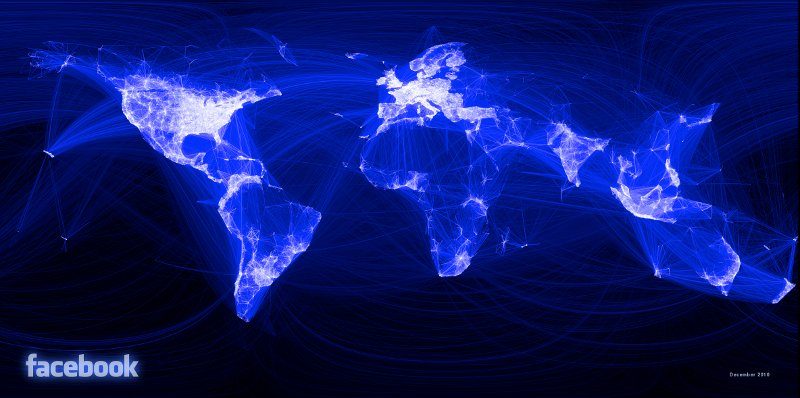
\includegraphics{figure/butler_facebook_2.jpg}
\caption{Iconic plot of Facebook friendship networks worldwide, by Paul
Butler}
\end{figure}

The impact of the map was to inspire the R community to produce more
ambitious graphics; a process fuelled by the increased demand for data
visualisation and the development of sophisticated packages, such as
ggplot2, that augment the basic plot functions of R. It is now the case
that R has become a key analysis and visualisation tool used by the
likes of Twitter, the New York Times and Google and thousands of
consultants, design houses and journalists. It is not longer the
preserve of academic research, with many graduate jobs listing R as a
desirable skill.

Finally, it is worth noting that while dedicated GIS programs handle
spatial data by default and display the results in a single way, there
are various options in R that must be decided by the user, for example
whether to use R's base graphics or a dedicated graphics package such as
ggplot2. On the other hand, the main benefits of R for spatial data
visualisation lie in the \emph{reproducibility} of its outputs, a
feature that we will be using to great effect in this chapter.

\subsubsection{R and reproducible research}

There is a drive towards transparent data and methods in academic
publishing. R encourages truly transparent and reproducible research by
enabling anyone with an R installation reproduce results described in a
previous paper. This process is facilitated by the RStudio software that
allows `live' R code and results to be embedded in documents.

\section{A practical primer on spatial data in R}

This section briefly introduces the input data and how they can be
loaded in R. It is a \emph{practical} chapter, so R code will be
provided that will allow the steps described to be reproduced on your
own computer.

The first stage, as with most GIS projects, is to obtain and load the
data. In this case, all the data has been uploaded to an on-line
repository that provides a detailed tutorial to accompany this Chapter:
\href{https://github.com/geocomPP/sdvwR/blob/master/sdv-tutorial.pdf?raw=true}{github.com/geocomPP/sdvwR}.
Upon visiting this page you will see many files: the pdf file is the
additional tutorial. To download the data, click on the ``Download ZIP''
button on the right, and unpack the folder to a sensible place on your
computer (e.g.~the Desktop). Explore the folder and try opening some of
the files, especially those from the sub-folder entitled ``data'': these
are the input files. For those new to R, we recom

In any data analysis project, spatial or otherwise, it is important to
have a strong understanding of the dataset before progressing. We will
see how data can be loaded into R (ready for the next section) and
exported to other formats.

\subsection{Loading spatial data in R}

R is able to import a very wide range of spatial data formats thanks to
its interface with the Geospatial Data Abstraction Library (GDAL). The
\texttt{rgdal} package makes this possible and it can be installed and
loaded by entering \texttt{install.packages("rgdal")} and
\texttt{library(rgdal)}. The former only needs to be typed once, as it
saves the data from the internet. The latter must be typed for each new
R session that requires the package.

The world map we use is available from the Natural Earth website and a
slightly modified version of it (entitled ``world'') is loaded using the
following code. A common problem preventing the data being loaded
correctly is that R is not in the correct \emph{working directory}.
Please refer to the online
\href{https://github.com/geocomPP/sdvwR/blob/master/sdv-tutorial.pdf?raw=true}{tutorial}
if this is an issue.

\begin{Shaded}
\begin{Highlighting}[]
\KeywordTok{library}\NormalTok{(rgdal)  }\CommentTok{# load the package (needs to be installed)}
\NormalTok{wrld <- }\KeywordTok{readOGR}\NormalTok{(}\StringTok{"data/"}\NormalTok{, }\StringTok{"world"}\NormalTok{)}
\KeywordTok{plot}\NormalTok{(wrld)}
\end{Highlighting}
\end{Shaded}
\begin{figure}[htbp]
\centering
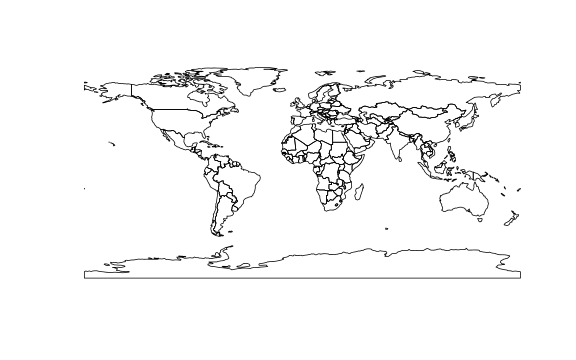
\includegraphics{figure/A_Basic_Map_of_the_World.png}
\caption{A Basic Map of the World}
\end{figure}

The above block of code loaded the rgdal library, created a new
\emph{object} called \texttt{wrld} and plotted this object to ensure it
is as we expect. This operation should be fast on most computers because
\texttt{wrld} is quite small. Spatial data can get very large indeed,
however. It is thus useful to understand how `large' the object you are
dealing with is, and know how to reduce unnecessary complexity in its
\emph{geometry} to make it more manageable to analyse, plot and store.
Fortunately, R makes this easy, as described in Section 2 of the
\href{https://github.com/geocomPP/sdvwR/blob/master/sdv-tutorial.pdf?raw=true}{tutorial}
that accompanies this Chapter. For now, let us continue with an even
more important topic: how R `sees' spatial data.

\subsection{How R `sees' spatial data}

Spatial datasets in R are saved in their own format, defined as
\texttt{Spatial} classes within the \texttt{sp} package. This data class
divides the spatial information into different \emph{slots} so the
attribute and geometry data are stored separately. This makes handling
spatial data in R memory efficient. For more detail on this topic, see
``The structure of spatial data in R'' in the on line tutorial. We will
see in the next section that this complex data structure can be
simplified in R using the \texttt{fortify} function.

For now, let us ask some basic questions about the \texttt{wrld} object,
using functions that would apply to any spatial dataset in R, to gain an
understanding of what we have loaded.

How many rows of attribute data are there? This query can be answered
using \texttt{nrow}:

\begin{Shaded}
\begin{Highlighting}[]
\KeywordTok{nrow}\NormalTok{(wrld)}
\end{Highlighting}
\end{Shaded}
\begin{verbatim}
## [1] 175
\end{verbatim}
What do the first 2 rows and 5 columns of attribute data contain? To
answer this question, we need to refer to the \texttt{data} slot of the
object using the \texttt{@} symbol and square brackets to define the
subset of the data to be displayed. In R, the rows are always referred
to before the comma within the square brackets and the column numbers
after. Try playing with the following line of code, for example by
removing the square brackets entirely:

\begin{Shaded}
\begin{Highlighting}[]
\NormalTok{wrld@data[}\DecValTok{1}\NormalTok{:}\DecValTok{2}\NormalTok{, }\DecValTok{1}\NormalTok{:}\DecValTok{5}\NormalTok{]}
\end{Highlighting}
\end{Shaded}
\begin{verbatim}
##   scalerank      featurecla labelrank  sovereignt sov_a3
## 0         1 Admin-0 country         3 Afghanistan    AFG
## 1         1 Admin-0 country         3      Angola    AGO
\end{verbatim}
The output shows that the first country in the \texttt{wrld} object is
Afganistan. Now that we have a basic understanding of the attributes of
the spatial dataset, and know where to look for more detailed
information about spatial data in R via the online tutorial, it is time
to move on to the topic of visualisation.

\section{Fundamentals of Spatial Data Visualisation}

Good maps depend on sound analysis and can have an enormous impact on
the understanding and communication of results. It has never been easier
to produce a map. The underlying data required are available in
unprecedented volumes and the technological capabilities of transforming
them into compelling maps and graphics are increasingly sophisticated
and straightforward to use. Data and software, however, only offer the
starting points of good spatial data visualisation since they need to be
refined and calibrated by the researchers seeking to communicate their
findings. In this section we will run through the features of a good
map. It is worth noting that not all good maps and graphics contain all
the features below -- they should simply be seen as suggestions rather
than firm principles.

Effective map making is hard process -- as Krygier and Wood (2011) put
it ``there is a lot to see, think about, and do'' (p6). It often comes
at the end of a period of intense data analysis and perhaps when the
priority is to get a paper finished and can therefore be rushed as a
result. The beauty of R (and other scripting languages) is the ability
to save code and simply re-run it with different data. Colours, map
adornments and other parameters can therefore be quickly applied, so it
is well worth creating a template script that adheres to best practice.

We have selected ggplot2 as our package of choice for the bulk of our
maps and spatial data visualisations because it has a number of these
elements at its core. The ``gg'' in its slightly odd name stands for
``Grammar of Graphics'', which is a set of rules developed by Leland
Wilkinson (2005) in a book of the same name. Grammar in the context of
graphics works in much the same way as it does in language - it provides
a structure. The structure is informed by both human perception and also
mathematics to ensure that the resulting visualisations are both
technically sound and comprehensible. By creating ggplot2, Hadley
Wickham, implemented these rules as well as developing ways in which
plots can be built up in layers (see Wickham, 2010). This layering
component is especially useful in the context of spatial data since it
is conceptually the same as map layers in Geographical Information
Systems (GIS).

First ensure that the necessary packages are installed and that R is in
the correct working directory (see above). Then load the ggplot2 package
used in this section.

\begin{Shaded}
\begin{Highlighting}[]
\KeywordTok{library}\NormalTok{(ggplot2)}
\end{Highlighting}
\end{Shaded}
We are going to use the previously loaded map of the world to
demonstrate some of the cartographic principles as they are introduced.
To establish the starting point, find the first 35 column names of the
\texttt{wrld} object:

\begin{Shaded}
\begin{Highlighting}[]
\KeywordTok{names}\NormalTok{(wrld@data)[}\DecValTok{1}\NormalTok{:}\DecValTok{35}\NormalTok{]}
\end{Highlighting}
\end{Shaded}
\begin{verbatim}
##  [1] "scalerank"  "featurecla" "labelrank"  "sovereignt" "sov_a3"    
##  [6] "adm0_dif"   "level"      "type"       "admin"      "adm0_a3"   
## [11] "geou_dif"   "geounit"    "gu_a3"      "su_dif"     "subunit"   
## [16] "su_a3"      "brk_diff"   "name"       "name_long"  "brk_a3"    
## [21] "brk_name"   "brk_group"  "abbrev"     "postal"     "formal_en" 
## [26] "formal_fr"  "note_adm0"  "note_brk"   "name_sort"  "name_alt"  
## [31] "mapcolor7"  "mapcolor8"  "mapcolor9"  "mapcolor13" "pop_est"
\end{verbatim}
You can see there are a lot of columns associated with this file.
Although we will keep all of them, we are only really interested in the
population estimate \texttt{("pop\_est")} field. Typing
\texttt{summary(wrld\$pop\_est)} provides basic descriptive statistics
on population.

Before progressing it is is worth reprojecting the data in order that
the population data can be seen better. The coordinate reference system
of the wrld shapefile is currently WGS84. This is the common latitude
and longitude format that all spatial software packages understand. From
a cartographic perspective the standard plots of this projection, of the
kind produced above, are not suitable since they heavily distort the
shapes of those countries further from the equator. Instead the Robinson
projection provides a good compromise between areal distortion and shape
preservation. We therefore project it as follows.

\begin{Shaded}
\begin{Highlighting}[]
\NormalTok{wrld.rob <- }\KeywordTok{spTransform}\NormalTok{(wrld, }\KeywordTok{CRS}\NormalTok{(}\StringTok{"+proj=robin"}\NormalTok{))}
\KeywordTok{plot}\NormalTok{(wrld.rob)}
\end{Highlighting}
\end{Shaded}
\begin{figure}[htbp]
\centering
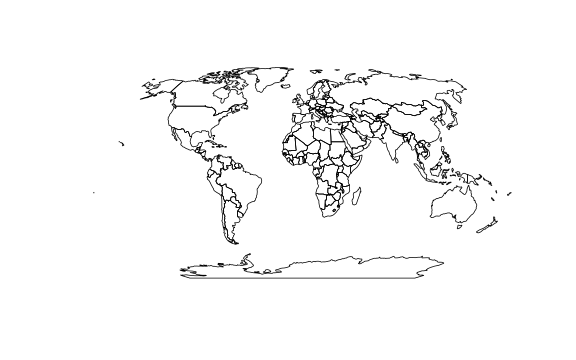
\includegraphics{figure/The_Robinson_Projection.png}
\caption{The Robinson Projection}
\end{figure}

\texttt{+proj=robin} refers to the Robinson projection. You will have
spotted from the plot that the countries in the world map are much
better proportioned.

We now need to \texttt{fortify} this spatial data to convert it into a
format that ggplot2 understands, we also use \texttt{merge} to re-attach
the attribute data that is lost in the fortify operation.

\begin{Shaded}
\begin{Highlighting}[]
\NormalTok{wrld.rob.f <- }\KeywordTok{fortify}\NormalTok{(wrld.rob, }\DataTypeTok{region =} \StringTok{"sov_a3"}\NormalTok{)}
\end{Highlighting}
\end{Shaded}
\begin{verbatim}
## Loading required package: rgeos
## rgeos version: 0.3-2, (SVN revision 413M)
##  GEOS runtime version: 3.3.9-CAPI-1.7.9 
##  Polygon checking: TRUE
\end{verbatim}
\begin{Shaded}
\begin{Highlighting}[]

\NormalTok{wrld.pop.f <- }\KeywordTok{merge}\NormalTok{(wrld.rob.f, wrld.rob@data, }\DataTypeTok{by.x =} \StringTok{"id"}\NormalTok{, }\DataTypeTok{by.y =} \StringTok{"sov_a3"}\NormalTok{)}
\end{Highlighting}
\end{Shaded}
The code below produces a map coloured by the population variable. It
demonstrates the sophistication of ggplot2 by first stringing together a
series of plot commands and assigning them to a single R object called
\texttt{map}. If you type \texttt{map} into the command line, R will
then execute the code and generate the plot. By simple specifing our
\texttt{fill} variable within the \texttt{aes()} part of the code and
then using the \texttt{geom\_polygon()} command ggplot2 will fill colour
the countries using a default colour pallette and auto-generated key. As
will be shown in the next section these defaults can be easily altered
to produce different looking maps.

\begin{Shaded}
\begin{Highlighting}[]
\NormalTok{map <- }\KeywordTok{ggplot}\NormalTok{(wrld.pop.f, }\KeywordTok{aes}\NormalTok{(long, lat, }\DataTypeTok{group =} \NormalTok{group, }\DataTypeTok{fill =} \NormalTok{pop_est)) + }\KeywordTok{geom_polygon}\NormalTok{() + }
    \KeywordTok{coord_equal}\NormalTok{() + }\KeywordTok{labs}\NormalTok{(}\DataTypeTok{x =} \StringTok{"Longitude"}\NormalTok{, }\DataTypeTok{y =} \StringTok{"Latitude"}\NormalTok{, }\DataTypeTok{fill =} \StringTok{"World Population"}\NormalTok{) + }
    \KeywordTok{ggtitle}\NormalTok{(}\StringTok{"World Population"}\NormalTok{)}

\NormalTok{map}
\end{Highlighting}
\end{Shaded}
\begin{figure}[htbp]
\centering
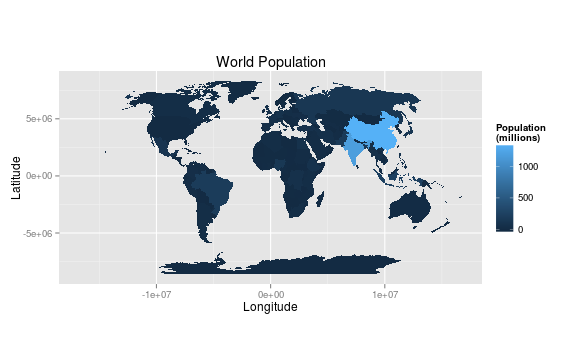
\includegraphics{figure/World_Population_Map.png}
\caption{World Population Map}
\end{figure}

\subsection{Colour and other aesthetics}

Colour has an enormous impact on how people will percieve a graphic.
Readers of a map come to it with a range of pre-conceptions about how
the world looks.

\subsubsection{Choropleth Maps}

ggplot2 knows the different between continuous and categorical (nominal)
data and will automatically assign the appropriate colour palettes when
producing choropleth maps such as the one above. The default colour
palettes are generally a good place to start but users may wish to vary
them for a whole host of reasons, such as the need to print in black and
white. The \texttt{scale\_fill\_} family of commands facilitate such
customisation. For categorical data \texttt{scale\_fill\_manual()} is a
useful command:

\begin{Shaded}
\begin{Highlighting}[]
\CommentTok{# Produce a map of continents}
\NormalTok{map.cont <- }\KeywordTok{ggplot}\NormalTok{(wrld.pop.f, }\KeywordTok{aes}\NormalTok{(long, lat, }\DataTypeTok{group =} \NormalTok{group, }\DataTypeTok{fill =} \NormalTok{continent)) + }
    \KeywordTok{geom_polygon}\NormalTok{() + }\KeywordTok{coord_equal}\NormalTok{() + }\KeywordTok{labs}\NormalTok{(}\DataTypeTok{x =} \StringTok{"Longitude"}\NormalTok{, }\DataTypeTok{y =} \StringTok{"Latitude"}\NormalTok{, }\DataTypeTok{fill =} \StringTok{"World Continents"}\NormalTok{) + }
    \KeywordTok{ggtitle}\NormalTok{(}\StringTok{"World Continents"}\NormalTok{)}

\CommentTok{# To see the default colours}
\NormalTok{map.cont}
\end{Highlighting}
\end{Shaded}
\begin{figure}[htbp]
\centering
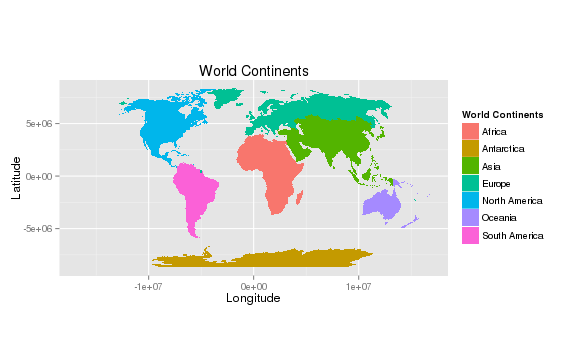
\includegraphics{figure/A_Map_of_the_Continents_Using_Default_Colours.png}
\caption{A Map of the Continents Using Default Colours}
\end{figure}

To change the colour scheme:

\begin{Shaded}
\begin{Highlighting}[]
\NormalTok{map.cont + }\KeywordTok{scale_fill_manual}\NormalTok{(}\DataTypeTok{values =} \KeywordTok{c}\NormalTok{(}\StringTok{"yellow"}\NormalTok{, }\StringTok{"red"}\NormalTok{, }\StringTok{"purple"}\NormalTok{, }\StringTok{"white"}\NormalTok{, }
    \StringTok{"orange"}\NormalTok{, }\StringTok{"blue"}\NormalTok{, }\StringTok{"green"}\NormalTok{, }\StringTok{"black"}\NormalTok{))}
\end{Highlighting}
\end{Shaded}
Whilst \texttt{scale\_fill\_continuous()} works with continuous
datasets:

\begin{Shaded}
\begin{Highlighting}[]
\CommentTok{# note the use of the 'map' object created earler}

\NormalTok{map + }\KeywordTok{scale_fill_continuous}\NormalTok{(}\DataTypeTok{low =} \StringTok{"white"}\NormalTok{, }\DataTypeTok{high =} \StringTok{"black"}\NormalTok{)}
\end{Highlighting}
\end{Shaded}
It is well worth looking at the \emph{Color Brewer} palettes developed
by Cynthia Brewer. These are designed to be colour blind safe and
perceptually uniform such that no one colour jumps out more than any
others. This latter characteristic is important when trying to produce
impartial maps. R has a package that contains the colour palettes and
these can be easily utlised by ggplot2.

\begin{Shaded}
\begin{Highlighting}[]
\KeywordTok{library}\NormalTok{(RColorBrewer)}
\CommentTok{# look at the help documents to see the palettes available. See}
\CommentTok{# http://colorbrewer2.org/}
\StringTok{`}\DataTypeTok{?}\StringTok{`}\NormalTok{(RColorBrewer)}
\CommentTok{# note the use of the scale_fill_gradientn() function rather than}
\CommentTok{# scale_fill_continuous() used above}
\NormalTok{map + }\KeywordTok{scale_fill_gradientn}\NormalTok{(}\DataTypeTok{colours =} \KeywordTok{brewer.pal}\NormalTok{(}\DecValTok{7}\NormalTok{, }\StringTok{"YlGn"}\NormalTok{))}
\end{Highlighting}
\end{Shaded}
In addition to altering the colour scale used to represent continuous
data it may also be desirable to adjust the breaks at which the colour
transitions occur. There are many ways to select both the optimum number
of breaks (i.e colour transitions) and the locations in the dataset at
which they occur. The \texttt{classINT} package contains many ways to
automatically create these breaks. We use the \texttt{grid.arrange}
function from the gridExtra package to display the maps side by side.

\begin{Shaded}
\begin{Highlighting}[]
\KeywordTok{library}\NormalTok{(classInt)}
\KeywordTok{library}\NormalTok{(gridExtra)}
\end{Highlighting}
\end{Shaded}
\begin{verbatim}
## Loading required package: grid
\end{verbatim}
\begin{Shaded}
\begin{Highlighting}[]

\CommentTok{# Specify how many breaks you want - generally this should be fewer than 7.}

\NormalTok{nbrks <- }\DecValTok{6}

\CommentTok{# Here quantiles are used to identify the breaks (note that we are using the}
\CommentTok{# original 'wrld.rob' object and not the 'wrld.rob@data$pop_est.f'). Use the}
\CommentTok{# help files to see the full range of options.}
\NormalTok{brks <- }\KeywordTok{classIntervals}\NormalTok{(wrld.rob@data$pop_est, }\DataTypeTok{n =} \NormalTok{nbrks, }\DataTypeTok{style =} \StringTok{"quantile"}\NormalTok{)}

\KeywordTok{print}\NormalTok{(brks)}
\end{Highlighting}
\end{Shaded}
\begin{verbatim}
## style: quantile
##        [-99,1990876)    [1990876,4615807)    [4615807,9059651) 
##                   29                   29                   29 
##   [9059651,16715999)  [16715999,40913584) [40913584,1.339e+09] 
##                   29                   29                   30
\end{verbatim}
\begin{Shaded}
\begin{Highlighting}[]

\CommentTok{# Now the breaks can be easily inserted into the code above for a range of}
\CommentTok{# colour palettes}
\NormalTok{YlGn <- map + }\KeywordTok{scale_fill_gradientn}\NormalTok{(}\DataTypeTok{colours =} \KeywordTok{brewer.pal}\NormalTok{(nbrks, }\StringTok{"YlGn"}\NormalTok{), }\DataTypeTok{breaks =} \KeywordTok{c}\NormalTok{(brks$brks))}

\NormalTok{PuBu <- map + }\KeywordTok{scale_fill_gradientn}\NormalTok{(}\DataTypeTok{colours =} \KeywordTok{brewer.pal}\NormalTok{(nbrks, }\StringTok{"PuBu"}\NormalTok{), }\DataTypeTok{breaks =} \KeywordTok{c}\NormalTok{(brks$brks))}

\KeywordTok{grid.arrange}\NormalTok{(YlGn, PuBu, }\DataTypeTok{ncol =} \DecValTok{2}\NormalTok{)}
\end{Highlighting}
\end{Shaded}
If you are not happy with the automatic methods for specifying breaks it
can also be done manually:

\begin{Shaded}
\begin{Highlighting}[]
\KeywordTok{library}\NormalTok{()}
\NormalTok{nbrks <- }\DecValTok{4}
\NormalTok{brks <- }\KeywordTok{c}\NormalTok{(}\FloatTok{1e+08}\NormalTok{, }\FloatTok{2.5e+08}\NormalTok{, }\FloatTok{5e+07}\NormalTok{, }\FloatTok{1e+09}\NormalTok{)}
\NormalTok{map + }\KeywordTok{scale_fill_gradientn}\NormalTok{(}\DataTypeTok{colours =} \KeywordTok{brewer.pal}\NormalTok{(nbrks, }\StringTok{"PuBu"}\NormalTok{), }\DataTypeTok{breaks =} \KeywordTok{c}\NormalTok{(brks))}
\end{Highlighting}
\end{Shaded}
\begin{figure}[htbp]
\centering
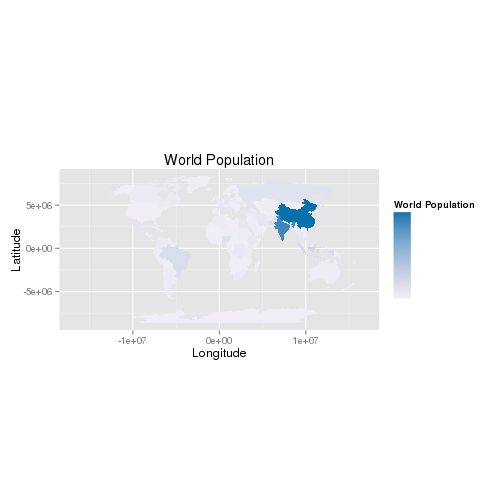
\includegraphics{figure/unnamed-chunk-6.png}
\caption{unnamed-chunk-6}
\end{figure}

There are many other ways to specify and alter the colours in ggplot2
and these are outlined in the help documentation.

If the map's purpose is to clearly communicate data then it is often
advisable to conform to conventions so as not to disorientate readers to
ensure they can focus on the key messages contained in the data. A good
example of this is the use of blue for bodies of water and green for
landmasses. The code example below generates two plots with our
wrld.pop.f object. The first colours the land blue and the sea (in this
case the background to the map) green and the second is more
conventional.

\begin{Shaded}
\begin{Highlighting}[]
\NormalTok{map2 <- }\KeywordTok{ggplot}\NormalTok{(wrld.pop.f, }\KeywordTok{aes}\NormalTok{(long, lat, }\DataTypeTok{group =} \NormalTok{group)) + }\KeywordTok{coord_equal}\NormalTok{()}

\NormalTok{blue <- map2 + }\KeywordTok{geom_polygon}\NormalTok{(}\DataTypeTok{fill =} \StringTok{"light blue"}\NormalTok{) + }\KeywordTok{theme}\NormalTok{(}\DataTypeTok{panel.background =} \KeywordTok{element_rect}\NormalTok{(}\DataTypeTok{fill =} \StringTok{"dark green"}\NormalTok{))}

\NormalTok{green <- map2 + }\KeywordTok{geom_polygon}\NormalTok{(}\DataTypeTok{fill =} \StringTok{"dark green"}\NormalTok{) + }\KeywordTok{theme}\NormalTok{(}\DataTypeTok{panel.background =} \KeywordTok{element_rect}\NormalTok{(}\DataTypeTok{fill =} \StringTok{"light blue"}\NormalTok{))}

\KeywordTok{grid.arrange}\NormalTok{(blue, green, }\DataTypeTok{ncol =} \DecValTok{2}\NormalTok{)}
\end{Highlighting}
\end{Shaded}
\begin{figure}[htbp]
\centering
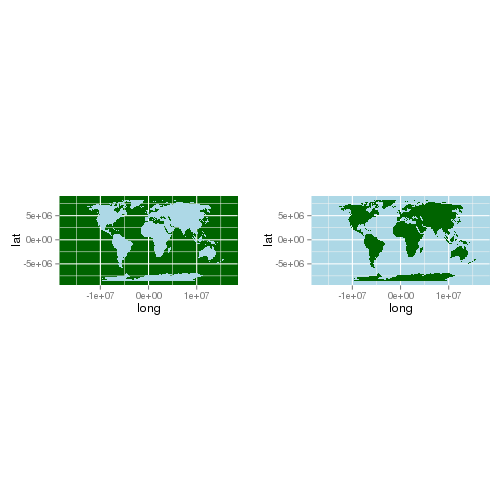
\includegraphics{figure/Conforming_to_Colour_Convention.png}
\caption{Conforming to Colour Convention}
\end{figure}

\subsubsection{Experimenting with line colour and line widths}

In addition to conforming to colour conventions, line colour and width
offer important parameters, which are often overlooked tools for
increasing the legibility of a graphic. As the code below demonstrates,
it is possible to adjust line colour through using the \texttt{colour}
parameter and the line width using the \texttt{lwd} parameter. The
impact of different line widths will vary depending on your screen size
and resolution. If you save the plot to pdf (or an image) then the size
at which you do this will also affect the line widths.

\begin{Shaded}
\begin{Highlighting}[]
\NormalTok{map3 <- map2 + }\KeywordTok{theme}\NormalTok{(}\DataTypeTok{panel.background =} \KeywordTok{element_rect}\NormalTok{(}\DataTypeTok{fill =} \StringTok{"light blue"}\NormalTok{))}

\NormalTok{yellow <- map3 + }\KeywordTok{geom_polygon}\NormalTok{(}\DataTypeTok{fill =} \StringTok{"dark green"}\NormalTok{, }\DataTypeTok{colour =} \StringTok{"yellow"}\NormalTok{)}

\NormalTok{black <- map3 + }\KeywordTok{geom_polygon}\NormalTok{(}\DataTypeTok{fill =} \StringTok{"dark green"}\NormalTok{, }\DataTypeTok{colour =} \StringTok{"black"}\NormalTok{)}

\NormalTok{thin <- map3 + }\KeywordTok{geom_polygon}\NormalTok{(}\DataTypeTok{fill =} \StringTok{"dark green"}\NormalTok{, }\DataTypeTok{colour =} \StringTok{"black"}\NormalTok{, }\DataTypeTok{lwd =} \FloatTok{0.1}\NormalTok{)}

\NormalTok{thick <- map3 + }\KeywordTok{geom_polygon}\NormalTok{(}\DataTypeTok{fill =} \StringTok{"dark green"}\NormalTok{, }\DataTypeTok{colour =} \StringTok{"black"}\NormalTok{, }\DataTypeTok{lwd =} \FloatTok{1.5}\NormalTok{)}

\KeywordTok{grid.arrange}\NormalTok{(yellow, black, thick, thin, }\DataTypeTok{ncol =} \DecValTok{2}\NormalTok{)}
\end{Highlighting}
\end{Shaded}
\begin{figure}[htbp]
\centering
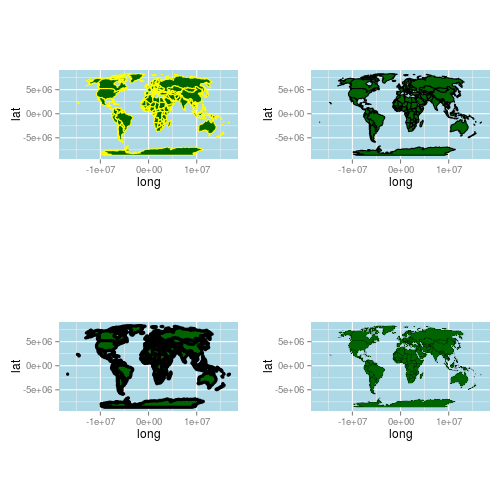
\includegraphics{figure/The_Impact_of_Line_Width.png}
\caption{The Impact of Line Width}
\end{figure}

There are other parameters such as layer transparency (use the
\texttt{alpha} parameter for this) that can be applied to all aspects of
the plot - both points, lines and polygons. Space does not permit their
full exploration here but more information is available from the many
online examples and the ggplot2 package documentation.

\subsection{Map Adornments and Annotations}

Map adornments and annotations are essential to orientate the viewer and
provide context; they include graticules, north arrows, scale bars and
data attribution. Not all are required on a single map, indeed it is
often best that they are used sparingly to avoid unecessary clutter
(Monkhouse and Wilkinson, 1971). With ggplot2 many of these are added
automatically but they can be customised.

\subsubsection{North arrow}

In the maps created so far, we have defined the \emph{aesthetics}
(\texttt{aes}) of the map in the foundation function \texttt{ggplot()}.
The result of this is that all subsequent layers are expected to have
the same variables. But what if we want to add a new layer from a
completely different dataset, for example to add a north arrow? To do
this, we must not add any arguments to the \texttt{ggplot} function,
only adding data sources one layer at a time:

Here we create an empty plot, meaning that each new layer must be given
its own dataset. While more code is needed in this example, it enables
much greater flexibility with regards to what can be included in new
layer contents. Another possibility is to use \texttt{geom\_segment()}
to add a rudimentary arrow (see \texttt{?geom\_segment} for
refinements):

\begin{Shaded}
\begin{Highlighting}[]
\KeywordTok{library}\NormalTok{(grid)  }\CommentTok{# needed for arrow}
\KeywordTok{ggplot}\NormalTok{() + }\KeywordTok{geom_polygon}\NormalTok{(}\DataTypeTok{data =} \NormalTok{wrld.pop.f, }\KeywordTok{aes}\NormalTok{(long, lat, }\DataTypeTok{group =} \NormalTok{group, }\DataTypeTok{fill =} \NormalTok{pop_est)) + }
    \KeywordTok{geom_line}\NormalTok{(}\KeywordTok{aes}\NormalTok{(}\DataTypeTok{x =} \KeywordTok{c}\NormalTok{(-}\FloatTok{1.3e+07}\NormalTok{, -}\FloatTok{1.3e+07}\NormalTok{), }\DataTypeTok{y =} \KeywordTok{c}\NormalTok{(}\DecValTok{0}\NormalTok{, }\FloatTok{5e+06}\NormalTok{)), }\DataTypeTok{arrow =} \KeywordTok{arrow}\NormalTok{()) + }
    \KeywordTok{coord_fixed}\NormalTok{()  }\CommentTok{# correct aspect ratio}
\end{Highlighting}
\end{Shaded}
\begin{figure}[htbp]
\centering
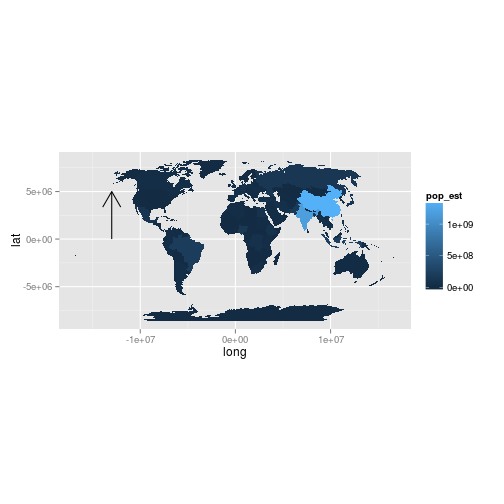
\includegraphics{figure/North_Arrow_Example.png}
\caption{North Arrow Example}
\end{figure}

\subsubsection{Scale bar}

ggplot2's scale bar capabilities are perhaps the least advanced element
of the package. For this example we use the \texttt{geom\_line()}
function to draw a line of approximately 1km in length using the
\texttt{lnd.f} object containing the London Boroughs discussed in
Section XXXX. This approach will only work if the spatial data are in a
projected coordinate system - in this case British National Grid - to
ensure there are no distortions as a result of the curvature of the
earth. In the case of the world map the distances at the equator in
terms of degrees east to west are very different from those further
north or south. Any line drawn using the the simple approach below would
therefore be inaccurate. For maps covering large areas - such as the
entire world - leaving the axis labels on will enable them to act as a
graticule to indicate distance.

\begin{Shaded}
\begin{Highlighting}[]
\KeywordTok{load}\NormalTok{(}\StringTok{"data/lnd.f.RData"}\NormalTok{)}
\KeywordTok{ggplot}\NormalTok{() + }\KeywordTok{geom_polygon}\NormalTok{(}\DataTypeTok{data =} \NormalTok{lnd.f, }\KeywordTok{aes}\NormalTok{(long, lat, }\DataTypeTok{group =} \NormalTok{group)) + }\KeywordTok{geom_line}\NormalTok{(}\KeywordTok{aes}\NormalTok{(}\DataTypeTok{x =} \KeywordTok{c}\NormalTok{(}\DecValTok{505000}\NormalTok{, }
    \DecValTok{515000}\NormalTok{), }\DataTypeTok{y =} \KeywordTok{c}\NormalTok{(}\DecValTok{158000}\NormalTok{, }\DecValTok{158000}\NormalTok{)), }\DataTypeTok{lwd =} \DecValTok{2}\NormalTok{) + }\KeywordTok{annotate}\NormalTok{(}\StringTok{"text"}\NormalTok{, }\DataTypeTok{label =} \StringTok{"10km"}\NormalTok{, }
    \DataTypeTok{x =} \DecValTok{510000}\NormalTok{, }\DataTypeTok{y =} \DecValTok{160000}\NormalTok{) + }\KeywordTok{coord_fixed}\NormalTok{()}
\end{Highlighting}
\end{Shaded}
\begin{figure}[htbp]
\centering
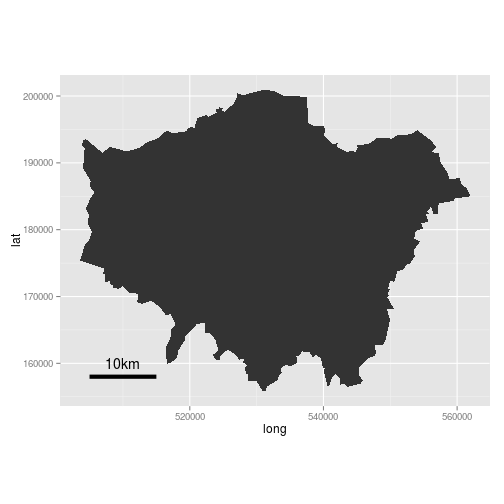
\includegraphics{figure/Scale_Bar_Example.png}
\caption{Scale Bar Example}
\end{figure}

\subsubsection{Legends}

Legends are added automatically but can be customised in a number of
ways. They are an important adornment of any map since they describe
what its colours mean. Try to select colour breaks that are easy to
follow and avoid labelling the legend with values that go to a large
number of significant figures. A few examples of legend customisation
are included below by way of introduction, but there are many more
examples avaialble in the \texttt{ggplot2} documentation.

\begin{Shaded}
\begin{Highlighting}[]
\CommentTok{# Position}
\NormalTok{map + }\KeywordTok{theme}\NormalTok{(}\DataTypeTok{legend.position =} \StringTok{"top"}\NormalTok{)}
\end{Highlighting}
\end{Shaded}
\begin{figure}[htbp]
\centering
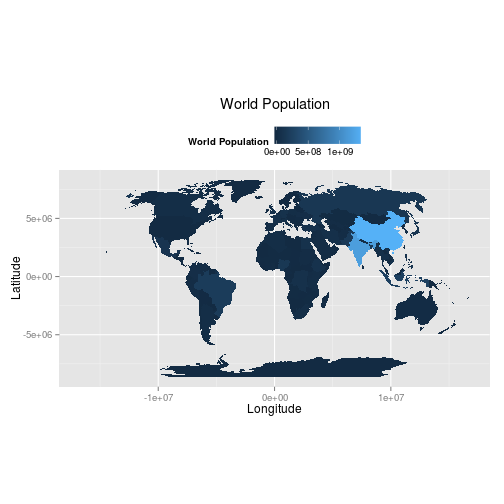
\includegraphics{figure/Formatting_the_Legend.png}
\caption{Formatting the Legend}
\end{figure}

As you can see, this added the legend in a new place. Many more options
for customization are available, as highlighed in the examples below.

\begin{Shaded}
\begin{Highlighting}[]
\CommentTok{# Title}
\NormalTok{map + }\KeywordTok{theme}\NormalTok{(}\DataTypeTok{legend.title =} \KeywordTok{element_text}\NormalTok{(}\DataTypeTok{colour =} \StringTok{"Red"}\NormalTok{, }\DataTypeTok{size =} \DecValTok{16}\NormalTok{, }\DataTypeTok{face =} \StringTok{"bold"}\NormalTok{))}

\CommentTok{# Label Font Size and Colour}
\NormalTok{map + }\KeywordTok{theme}\NormalTok{(}\DataTypeTok{legend.text =} \KeywordTok{element_text}\NormalTok{(}\DataTypeTok{colour =} \StringTok{"blue"}\NormalTok{, }\DataTypeTok{size =} \DecValTok{16}\NormalTok{, }\DataTypeTok{face =} \StringTok{"italic"}\NormalTok{))}

\CommentTok{# Border and background box}
\NormalTok{map + }\KeywordTok{theme}\NormalTok{(}\DataTypeTok{legend.background =} \KeywordTok{element_rect}\NormalTok{(}\DataTypeTok{fill =} \StringTok{"gray90"}\NormalTok{, }\DataTypeTok{size =} \FloatTok{0.5}\NormalTok{, }\DataTypeTok{linetype =} \StringTok{"dotted"}\NormalTok{))}
\end{Highlighting}
\end{Shaded}
\subsection{Adding Basemaps To Your Plots}

The development of the ggmap package has enabled the simple use of
online mapping services such as Google Maps and OpenStreetMap for base
maps. Using image tiles from these services spatial data can be placed
in context as users can easily orientate themselves to streets and
landmarks.

For this example we are going to use the shapefile of London sports
participation introduced in Section 2. The data were originally
projected to British National Grid (BNG) which is not compatible with
the online map services used in the following examples. It therefore
needs reprojecting - a step we completed earlier. The reprojected file
can be loaded as follows:

\begin{Shaded}
\begin{Highlighting}[]
\KeywordTok{load}\NormalTok{(}\StringTok{"data/lnd.wgs84.RData"}\NormalTok{)}
\end{Highlighting}
\end{Shaded}
The first job is to calculate the bounding box (bb for short) of the
\texttt{lnd.wgs84} object to identify the geographic extent of the map.
This information is used to request the appropriate map tiles from the
map service of our choice. This process is conceptually the same as the
size of your web browser or smartphone screen when using Google maps for
navigation. The first line of code in the snippet below retrieves the
bounding box and the two that follow add 5\% so there is a little space
around the edges of the data to be plotted.

\begin{Shaded}
\begin{Highlighting}[]
\NormalTok{b <- }\KeywordTok{bbox}\NormalTok{(lnd.wgs84)}
\NormalTok{b[}\DecValTok{1}\NormalTok{, ] <- (b[}\DecValTok{1}\NormalTok{, ] - }\KeywordTok{mean}\NormalTok{(b[}\DecValTok{1}\NormalTok{, ])) * }\FloatTok{1.05} \NormalTok{+ }\KeywordTok{mean}\NormalTok{(b[}\DecValTok{1}\NormalTok{, ])}
\NormalTok{b[}\DecValTok{2}\NormalTok{, ] <- (b[}\DecValTok{2}\NormalTok{, ] - }\KeywordTok{mean}\NormalTok{(b[}\DecValTok{2}\NormalTok{, ])) * }\FloatTok{1.05} \NormalTok{+ }\KeywordTok{mean}\NormalTok{(b[}\DecValTok{2}\NormalTok{, ])}
\CommentTok{# scale longitude and latitude (increase bb by 5% for plot) replace 1.05}
\CommentTok{# with 1.xx for an xx% increase in the plot size}
\end{Highlighting}
\end{Shaded}
This is then fed into the \texttt{get\_map} function as the location
parameter. The syntax below contains 2 functions. \texttt{ggmap} is
required to produce the plot and provides the base map data.

\begin{Shaded}
\begin{Highlighting}[]
\KeywordTok{library}\NormalTok{(ggmap)}

\NormalTok{lnd.b1 <- }\KeywordTok{ggmap}\NormalTok{(}\KeywordTok{get_map}\NormalTok{(}\DataTypeTok{location =} \NormalTok{b))}
\end{Highlighting}
\end{Shaded}
\begin{verbatim}
## Warning: bounding box given to google - spatial extent only approximate.
\end{verbatim}
\texttt{ggmap} follows the same syntax structures as ggplot2 and so can
easily be integrated with the other examples included here. First
\texttt{fortify} the \texttt{lnd.wgs84} object and then merge with the
required attribute data.

\begin{Shaded}
\begin{Highlighting}[]
\NormalTok{lnd.wgs84.f <- }\KeywordTok{fortify}\NormalTok{(lnd.wgs84, }\DataTypeTok{region =} \StringTok{"ons_label"}\NormalTok{)}
\NormalTok{lnd.wgs84.f <- }\KeywordTok{merge}\NormalTok{(lnd.wgs84.f, lnd.wgs84@data, }\DataTypeTok{by.x =} \StringTok{"id"}\NormalTok{, }\DataTypeTok{by.y =} \StringTok{"ons_label"}\NormalTok{)}
\end{Highlighting}
\end{Shaded}
We can now overlay this on our base map using the
\texttt{geom\_polygon()} function.

\begin{Shaded}
\begin{Highlighting}[]
\NormalTok{lnd.b1 + }\KeywordTok{geom_polygon}\NormalTok{(}\DataTypeTok{data =} \NormalTok{lnd.wgs84.f, }\KeywordTok{aes}\NormalTok{(}\DataTypeTok{x =} \NormalTok{long, }\DataTypeTok{y =} \NormalTok{lat, }\DataTypeTok{group =} \NormalTok{group, }
    \DataTypeTok{fill =} \NormalTok{Partic_Per), }\DataTypeTok{alpha =} \FloatTok{0.5}\NormalTok{)}
\end{Highlighting}
\end{Shaded}
The resulting map looks reasonable, but it would be improved with a
simpler base map in black and white. A design firm called \emph{stamen}
provide the tiles we need and they can be brought into the plot with the
\texttt{get\_map} function:

\begin{Shaded}
\begin{Highlighting}[]
\NormalTok{lnd.b2 <- }\KeywordTok{ggmap}\NormalTok{(}\KeywordTok{get_map}\NormalTok{(}\DataTypeTok{location =} \NormalTok{b, }\DataTypeTok{source =} \StringTok{"stamen"}\NormalTok{, }\DataTypeTok{maptype =} \StringTok{"toner"}\NormalTok{, }
    \DataTypeTok{crop =} \NormalTok{T))  }\CommentTok{#note the addition of the maptype parameter.}
\end{Highlighting}
\end{Shaded}
We can then produce the plot as before.

\begin{Shaded}
\begin{Highlighting}[]
\NormalTok{lnd.b2 + }\KeywordTok{geom_polygon}\NormalTok{(}\DataTypeTok{data =} \NormalTok{lnd.wgs84.f, }\KeywordTok{aes}\NormalTok{(}\DataTypeTok{x =} \NormalTok{long, }\DataTypeTok{y =} \NormalTok{lat, }\DataTypeTok{group =} \NormalTok{group, }
    \DataTypeTok{fill =} \NormalTok{Partic_Per), }\DataTypeTok{alpha =} \FloatTok{0.5}\NormalTok{)}
\end{Highlighting}
\end{Shaded}
This produces a much clearer map and enables readers to focus on the
data rather than the basemap. Spatial polygons are not the only data
types compatible with \texttt{ggmap} - you can use any plot type and set
of parameters available in \texttt{ggplot2}, making it an ideal
companion package for spatial data visualisation.

\section{A Final Example}

Here we present a final example that draws upon the many advanced
concepts discussed in this chapter to produce a map of 18th Century
Shipping flows. The data have been obtained from the CLIWOC project and
they represent a sample of digitised ships' logs from the 18th Century.
We are using a very small sample of the the full dataset, which is
available from here: http://pendientedemigracion.ucm.es/info/cliwoc/.
The example has been chosen to demonstrate a range of capabilities
within ggplot2 and the ways in which they can be applied to produce
high-quality maps with only a few lines of code. We end by showing how
the maps can be animated to chart the routes over time and the ability
of R to produce many maps very quickly.

As always, the first step is to load in the required packages and
datasets. Here we are using the png package to load in a series of map
annotations. These have been created in image editing software and will
add a historic feel to the map. We are also loading in a World boundary
shapefile and the shipping data itself.

\begin{Shaded}
\begin{Highlighting}[]
\KeywordTok{library}\NormalTok{(rgdal)}
\KeywordTok{library}\NormalTok{(ggplot2)}
\KeywordTok{library}\NormalTok{(png)}
\NormalTok{wrld <- }\KeywordTok{readOGR}\NormalTok{(}\StringTok{"data/"}\NormalTok{, }\StringTok{"ne_110m_admin_0_countries"}\NormalTok{)}
\end{Highlighting}
\end{Shaded}
\begin{verbatim}
## OGR data source with driver: ESRI Shapefile 
## Source: "data/", layer: "ne_110m_admin_0_countries"
## with 177 features and 63 fields
## Feature type: wkbPolygon with 2 dimensions
\end{verbatim}
\begin{Shaded}
\begin{Highlighting}[]
\NormalTok{btitle <- }\KeywordTok{readPNG}\NormalTok{(}\StringTok{"figure/brit_titles.png"}\NormalTok{)}
\NormalTok{compass <- }\KeywordTok{readPNG}\NormalTok{(}\StringTok{"figure/windrose.png"}\NormalTok{)}
\NormalTok{bdata <- }\KeywordTok{read.csv}\NormalTok{(}\StringTok{"data/british_shipping_example.csv"}\NormalTok{)}
\end{Highlighting}
\end{Shaded}
If you look at the first few lines in the \texttt{bdata} object you will
see there are 7 columns with each row representing a single point on the
ships course. The year of the journey and the nationality of the ship
are also included. The final 3 columns are identifiers that are used
later to group the coordinate points together into the paths that
ggplot2 plots.

We first specify some plot parameters that remove the axis labels.

\begin{Shaded}
\begin{Highlighting}[]
\NormalTok{xquiet <- }\KeywordTok{scale_x_continuous}\NormalTok{(}\StringTok{""}\NormalTok{, }\DataTypeTok{breaks =} \OtherTok{NULL}\NormalTok{)}
\NormalTok{yquiet <- }\KeywordTok{scale_y_continuous}\NormalTok{(}\StringTok{""}\NormalTok{, }\DataTypeTok{breaks =} \OtherTok{NULL}\NormalTok{)}
\NormalTok{quiet <- }\KeywordTok{list}\NormalTok{(xquiet, yquiet)}
\end{Highlighting}
\end{Shaded}
The next step is to \texttt{fortify} the World coastlines and create the
base plot. This sets the extents of the plot window and provides the
blank canvas on which we will build up the layers. The first layer
created is the wrld object; the code is wrapped in \texttt{c()} to
prevent it from executing by simply storing it as the plot's parameters.

\begin{Shaded}
\begin{Highlighting}[]
\NormalTok{wrld.f <- }\KeywordTok{fortify}\NormalTok{(wrld, }\DataTypeTok{region =} \StringTok{"sov_a3"}\NormalTok{)}
\NormalTok{base <- }\KeywordTok{ggplot}\NormalTok{(wrld.f, }\KeywordTok{aes}\NormalTok{(}\DataTypeTok{x =} \NormalTok{long, }\DataTypeTok{y =} \NormalTok{lat))}
\NormalTok{wrld <- }\KeywordTok{c}\NormalTok{(}\KeywordTok{geom_polygon}\NormalTok{(}\KeywordTok{aes}\NormalTok{(}\DataTypeTok{group =} \NormalTok{group), }\DataTypeTok{size =} \FloatTok{0.1}\NormalTok{, }\DataTypeTok{colour =} \StringTok{"black"}\NormalTok{, }\DataTypeTok{fill =} \StringTok{"#D6BF86"}\NormalTok{, }
    \DataTypeTok{data =} \NormalTok{wrld.f, }\DataTypeTok{alpha =} \DecValTok{1}\NormalTok{))}
\end{Highlighting}
\end{Shaded}
To see the result of this simply type:

\begin{Shaded}
\begin{Highlighting}[]
\NormalTok{base + wrld + }\KeywordTok{coord_fixed}\NormalTok{()}
\end{Highlighting}
\end{Shaded}
\begin{figure}[htbp]
\centering
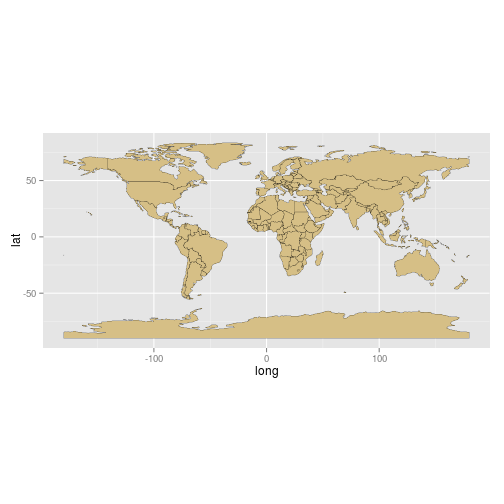
\includegraphics{figure/World_Map.png}
\caption{World Map}
\end{figure}

The code snipped below creates the plot layer containing the the
shipping routes. The \texttt{geom\_path()} function is used to string
together the coordinates into the routes. You can see within the
\texttt{aes()} component we have specified long and lat plus pasted
together the trp and \texttt{group.regroup} variables to identify the
unique paths.

\begin{Shaded}
\begin{Highlighting}[]
\NormalTok{route <- }\KeywordTok{c}\NormalTok{(}\KeywordTok{geom_path}\NormalTok{(}\KeywordTok{aes}\NormalTok{(long, lat, }\DataTypeTok{group =} \KeywordTok{paste}\NormalTok{(bdata$trp, bdata$group.regroup, }
    \DataTypeTok{sep =} \StringTok{"."}\NormalTok{)), }\DataTypeTok{colour =} \StringTok{"#0F3B5F"}\NormalTok{, }\DataTypeTok{size =} \FloatTok{0.2}\NormalTok{, }\DataTypeTok{data =} \NormalTok{bdata, }\DataTypeTok{alpha =} \FloatTok{0.5}\NormalTok{, }
    \DataTypeTok{lineend =} \StringTok{"round"}\NormalTok{))}
\end{Highlighting}
\end{Shaded}
We now have all we need to generate the final plot by building the
layers together with the \texttt{+} sign as shown in the code below. The
first 3 arguments are the plot layers, and the parameters within
\texttt{theme()} are changing the background colour to sea blue.
\texttt{annotation\_raster()} plots the png map adornments loaded in
earlier- this requires the bounding box of each image to be specified.
In this case we use latitude and longitude (in WGS84) and we can use
these paramrters to change the png's position and also its size. The
final two arguments fix the aspect ratio of the plot and remove the axis
labels.

\begin{Shaded}
\begin{Highlighting}[]
\NormalTok{base + route + wrld + }\KeywordTok{theme}\NormalTok{(}\DataTypeTok{panel.background =} \KeywordTok{element_rect}\NormalTok{(}\DataTypeTok{fill =} \StringTok{"#BAC4B9"}\NormalTok{, }
    \DataTypeTok{colour =} \StringTok{"black"}\NormalTok{)) + }\KeywordTok{annotation_raster}\NormalTok{(btitle, }\DataTypeTok{xmin =} \DecValTok{30}\NormalTok{, }\DataTypeTok{xmax =} \DecValTok{140}\NormalTok{, }\DataTypeTok{ymin =} \DecValTok{51}\NormalTok{, }
    \DataTypeTok{ymax =} \DecValTok{87}\NormalTok{) + }\KeywordTok{annotation_raster}\NormalTok{(compass, }\DataTypeTok{xmin =} \DecValTok{65}\NormalTok{, }\DataTypeTok{xmax =} \DecValTok{105}\NormalTok{, }\DataTypeTok{ymin =} \DecValTok{25}\NormalTok{, }
    \DataTypeTok{ymax =} \DecValTok{65}\NormalTok{) + }\KeywordTok{coord_equal}\NormalTok{() + quiet}
\end{Highlighting}
\end{Shaded}
\begin{figure}[htbp]
\centering
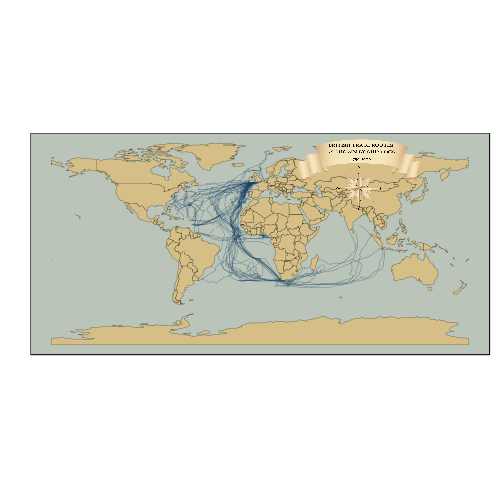
\includegraphics{figure/World_Shipping.png}
\caption{World Shipping}
\end{figure}

In the plot example we have chosen the colours carefully to give the
appearance of a historic map. An alternative approach could be to use a
satellite image as a base map. It is possible to use the readPNG
function to import NASA's ``Blue Marble'' image for this purpose. Given
that the route information is the same projection as the image it is
very straightforward to set the image extent to span -180 to 180 degrees
and -90 to 90 degrees and have it align with the shipping data.
Producing the plot is accomplished using the code below. This offers a
good example of where functionality designed without spatial data in
mind can be harnessed for the purposes of producing interesting maps.
Once you have produced the plot, alter the code to recolour the shipping
routes to make them appear more clearly against the blue marble
background.

\begin{Shaded}
\begin{Highlighting}[]
\NormalTok{earth <- }\KeywordTok{readPNG}\NormalTok{(}\StringTok{"figure/earth_raster.png"}\NormalTok{)}

\NormalTok{base + }\KeywordTok{annotation_raster}\NormalTok{(earth, }\DataTypeTok{xmin =} \NormalTok{-}\DecValTok{180}\NormalTok{, }\DataTypeTok{xmax =} \DecValTok{180}\NormalTok{, }\DataTypeTok{ymin =} \NormalTok{-}\DecValTok{90}\NormalTok{, }\DataTypeTok{ymax =} \DecValTok{90}\NormalTok{) + }
    \NormalTok{route + }\KeywordTok{theme}\NormalTok{(}\DataTypeTok{panel.background =} \KeywordTok{element_rect}\NormalTok{(}\DataTypeTok{fill =} \StringTok{"#BAC4B9"}\NormalTok{, }\DataTypeTok{colour =} \StringTok{"black"}\NormalTok{)) + }
    \KeywordTok{annotation_raster}\NormalTok{(btitle, }\DataTypeTok{xmin =} \DecValTok{30}\NormalTok{, }\DataTypeTok{xmax =} \DecValTok{140}\NormalTok{, }\DataTypeTok{ymin =} \DecValTok{51}\NormalTok{, }\DataTypeTok{ymax =} \DecValTok{87}\NormalTok{) + }
    \KeywordTok{annotation_raster}\NormalTok{(compass, }\DataTypeTok{xmin =} \DecValTok{65}\NormalTok{, }\DataTypeTok{xmax =} \DecValTok{105}\NormalTok{, }\DataTypeTok{ymin =} \DecValTok{25}\NormalTok{, }\DataTypeTok{ymax =} \DecValTok{65}\NormalTok{) + }
    \KeywordTok{coord_equal}\NormalTok{() + quiet}
\end{Highlighting}
\end{Shaded}
\begin{figure}[htbp]
\centering
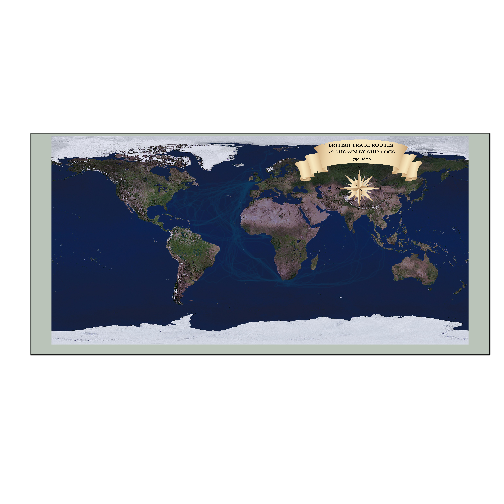
\includegraphics{figure/World_Shipping_with_raster_background.png}
\caption{World Shipping with raster background}
\end{figure}

\section{Conclusions}

There are an almost infinite number of different combinations colours,
adornments and line widths that could be applied to a map, so take
inspiration from maps and graphics you have seen and liked. The process
is an iterative one, it will take multiple attempts to get right. Show
your map to friends and colleagues - all will have an opinion but don't
be afraid to stand by the decisions you have taken. To give your maps a
final polish you may wish to export them as a pdf using the
\texttt{ggsave()} function and importing them into a vector graphics
package such as Adobe Illustrator or Inkscape.

The beauty of producing maps in a programming environment as opposed to
the GUI offered by the majority of GIS software packages lies in the
fact that each line of code can be easily adapted to a different
dataset. Users can therefore create a series of scripts that act as
templates and simply call them when required. This saves a huge amount
of time and has the added advantage that all outputs will have a
consistent style and thus offer more professional looking publications.

This chapter has covered a large number of techniques and approaches for
the preparation, analysis and visualisation of spatial data in R. Whilst
it only covers the tip of the iceberg in terms of R's capabilities, it
does lay the foundations to the use of the multitude of other spatial
data packages available. These can be discovered online and through the
help documentation and other chapters provided by the R community. By
utilising the data visualisation techniques and examples of best
practice we have covered it is hoped that you will be able to
communicate your results in a compelling and effective way without the
need for the repetitive ``pointing and clicking'' required of many GIS
packages; you can now tweak colours and other aspects of the plots
without the need to start from scratch each time an iterative
improvement is required. As the R community grows so will its range of
applications and available packages so there will be many exciting
opportunities ahead to improve on what is presented here.

\section{References}

Bivand, R., \& Gebhardt, A. (2000). Implementing functions for spatial
statistical analysis using the R language. Journal of Geographical
Systems, 2(3), 307--317.

Bivand, R. S., Pebesma, E. J., \& Rubio, V. G. (2013). Applied spatial
data: analysis with R. Springer.

Burrough, P. A. \& McDonnell, R. A. (1998). Principals of Geographic
Information Systems (revised edition). Clarendon Press, Oxford.

Goodchild, M. F. (2007). Citizens as sensors: the world of volunteered
geography. GeoJournal, 69(4), 211--221.

Harris, R. (2012). A Short Introduction to R.
\href{http://www.social-statistics.org/}{social-statistics.org}.

Kabacoff, R. (2011). R in Action. Manning Publications Co.

Krygier, J. Wood, D. 2011. Making Maps: A Visual Guide to Map Design for
GIS (2nd Ed.). New York: The Guildford Press.

Longley, P., Goodchild, M. F., Maguire, D. J., \& Rhind, D. W. (2005).
Geographic information systems and science. John Wiley \& Sons.

Monkhouse, F.J. and Wilkinson, H. R. 1973. Maps and Diagrams Their
Compilation and Construction (3rd Edition, reprinted with revisions).
London: Methuen \& Co Ltd.

Ramsey, P., \& Dubovsky, D. (2013). Geospatial Software's Open Future.
GeoInformatics, 16(4).

Sherman, G. (2008). Desktop GIS: Mapping the Planet with Open Source
Tools. Pragmatic Bookshelf.

Torfs and Brauer (2012). A (very) short Introduction to R. The
Comprehensive R Archive Network.

Venables, W. N., Smith, D. M., \& Team, R. D. C. (2013). An introduction
to R. The Comprehensive R Archive Network (CRAN). Retrieved from
http://cran.ma.imperial.ac.uk/doc/manuals/r-devel/R-intro.pdf .

Wickham, H. (2009). ggplot2: elegant graphics for data analysis.
Springer.

Wickham, H. 2010. A Layered Grammar of Graphics. American Statistical
Association, Institute of Mathematics Statistics and Interface
Foundation of North America Journal of Computational and Graphical
Statistics. 19, 1: 3-28

\section{Endnotes}

\begin{enumerate}[1.]
\item
  ``What kind of a name is R?'' common question. R's name originates
  from the creators of R, Ross Ihaka and Robert Gentleman. R is an open
  source implementation of the statistical programming language S, so
  its name is also a play on words that makes implicit reference to
  this.
\item
  R is notoriously difficult to search for on major search engines, as
  it is such a common letter with many other uses beyond the name of a
  statistical programming language. This should not be a deterrent, as R
  has a wealth of excellent online resources. To overcome the issue, you
  can either be more specific with the search term (e.g. ``R spatial
  statistics'') or use an R specific search engine such as
  \href{http://www.rseek.org/}{rseek.org}. You can also search of online
  help \emph{from within R} using the command \texttt{RSiteSearch}. E.g.
  \texttt{RSiteSearch("spatial statistics")}. Experiment and see which
  you prefer!
\end{enumerate}
\begin{Shaded}
\begin{Highlighting}[]
\KeywordTok{source}\NormalTok{(}\StringTok{"md2pdf.R"}\NormalTok{)  }\CommentTok{# convert chapter to tex}
\end{Highlighting}
\end{Shaded}

\end{document}
